\documentclass[a4paper,12pt]{article}
\usepackage[a4paper, top=2cm,bottom=2cm,right=2cm,left=2cm]{geometry}

\usepackage{bm,xcolor,mathdots,latexsym,amsfonts,amsthm,amsmath,
					mathrsfs,graphicx,cancel,tikz-cd,hyperref,booktabs,caption,amssymb,amssymb,wasysym}
\hypersetup{colorlinks=true,linkcolor=blue}
\usepackage[italian]{babel}
\usepackage[T1]{fontenc}
\usepackage[utf8]{inputenc}
\newcommand{\s}[1]{\left\{ #1 \right\}}
\newcommand{\sbarra}{\backslash} %% \ 
\newcommand{\ds}{\displaystyle} 
\newcommand{\alla}{^}  
\newcommand{\implica}{\Rightarrow}
\newcommand{\iimplica}{\Leftarrow}
\newcommand{\ses}{\Leftrightarrow} %se e solo se
\newcommand{\tc}{\quad \text{ t. c .} \quad } % tale che 
\newcommand{\spazio}{\vspace{0.5 cm}}
\newcommand{\bbianco}{\textcolor{white}{,}}
\newcommand{\bianco}{\textcolor{white}{,} \\}% per andare a capo dopo 																					definizioni teoremi ...


% campi 
\newcommand{\N}{\mathbb{N}} 
\newcommand{\R}{\mathbb{R}}
\newcommand{\Q}{\mathbb{Q}}
\newcommand{\Z}{\mathbb{Z}}
\newcommand{\K}{\mathbb{K}} 
\newcommand{\C}{\mathbb{C}}
\newcommand{\F}{\mathbb{F}}
\newcommand{\p}{\mathbb{P}}

%GEOMETRIA
\newcommand{\B}{\mathfrak{B}} %Base B
\newcommand{\D}{\mathfrak{D}}%Base D
\newcommand{\RR}{\mathfrak{R}}%Base R 
\newcommand{\Can}{\mathfrak{C}}%Base canonica
\newcommand{\Rif}{\mathfrak{R}}%Riferimento affine
\newcommand{\AB}{M_\D ^\B }% matrice applicazione rispetto alla base B e D 
\newcommand{\vett}{\overrightarrow}
\newcommand{\sd}{\sim_{SD}}%relazione sx dx
\newcommand{\nvett}{v_1, \, \dots , \, v_n} % v1 ... vn
\newcommand{\ncomb}{a_1 v_1 + \dots + a_n v_n} %a1 v1 + ... +an vn
\newcommand{\nrif}{P_1, \cdots , P_n} 
\newcommand{\bidu}{\left( V^\star \right)^\star}

\newcommand{\udis}{\amalg}
\newcommand{\ric}{\mathfrak{U}}
\newcommand{\inclu}{\hookrightarrow }
%ALGEBRA

\newcommand{\semidir}{\rtimes}%semidiretto
\newcommand{\W}{\Omega}
\newcommand{\norma}{\vert \vert }
\newcommand{\bignormal}{\left\vert \left\vert}
\newcommand{\bignormar}{\right\vert \right\vert}
\newcommand{\normale}{\triangleleft}
\newcommand{\nnorma}{\vert \vert \, \cdot \, \vert \vert}
\newcommand{\dt}{\, \mathrm{d}t}
\newcommand{\dz}{\, \mathrm{d}z}
\newcommand{\dx}{\, \mathrm{d}x}
\newcommand{\dy}{\, \mathrm{d}y}
\newcommand{\amma}{\gamma}
\newcommand{\inv}[1]{#1^{-1}}
\newcommand{\az}{\centerdot}
\newcommand{\ammasol}[1]{\tilde{\gamma}_{\tilde{#1}}}
\newcommand{\pror}[1]{\mathbb{P}^#1 (\R)}
\newcommand{\proc}[1]{\mathbb{P}^#1(\C)}
\newcommand{\sol}[2]{\widetilde{#1}_{\widetilde{#2}}}
\newcommand{\bsol}[3]{\left(\widetilde{#1}\right)_{\widetilde{#2}_{#3}}}
\newcommand{\norm}[1]{\left\vert\left\vert #1 \right\vert \right\vert}
\newcommand{\abs}[1]{\left\vert #1 \right\vert }
\newcommand{\ris}[2]{#1_{\vert #2}}
\newcommand{\vp}{\varphi}
\newcommand{\vt}{\vartheta}
\newcommand{\wt}[1]{\widetilde{#1}}
\newcommand{\pr}[2]{\frac{\partial \, #1}{\partial\, #2}}%derivata parziale
%per creare teoremi, dimostrazioni ... 
\theoremstyle{plain}
\newtheorem{thm}{Teorema}[section] 
\newtheorem{ese}[thm]{Esempio} 
\newtheorem{ex}[thm]{Esercizio} 
\newtheorem{fatti}[thm]{Fatti}
\newtheorem{fatto}[thm]{Fatto}

\newtheorem{cor}[thm]{Corollario} 
\newtheorem{lem}[thm]{Lemma} 
\newtheorem{al}[thm]{Algoritmo}
\newtheorem{prop}[thm]{Proposizione} 
\theoremstyle{definition} 
\newtheorem{defn}{Definizione}[section] 
\newcommand{\intt}[2]{int_{#1}^{#2}}
\theoremstyle{remark} 
\newtheorem{oss}{Osservazione} 
\newcommand{\di }{\, \mathrm{d}}
\newcommand{\tonde}[1]{\left( #1 \right)}
\newcommand{\quadre}[1]{\left[ #1 \right]}
\newcommand{\w}{\omega}

% diagrammi commutativi tikzcd
% per leggere la documentazione texdoc

\begin{document}
\textbf{Lezione del 6 maggio}
\begin{ese}\label{ex1} Siano $A,B,C,D$ in $\p^2( \K)$ in posizione generale, consideriamo i punti
$$ P=L(A,B) \cap L(C,D) \quad Q = L(A,C) \cap L(B,D) \quad R=L(A,D) \cap L(B,C)$$
I punti $P,Q,R$ sono allineati?\\
Da un lemma sappiamo che $A,B,C,D$ determinano un riferimento proiettivo in cui
$$ A=[e_0] \, \, B=[e_1] \, \, C=[e_2]\, \, D=[e_0+e_1+e_2]$$
determiniamo le equazioni parametriche delle rette definite sopra
$$ L(A,B) :  \det \begin{pmatrix} 1 & 0 & x_0 \\
													 0 & 1 & x_1\\
 													0 & 0 & x_2
\end{pmatrix} =0 \quad \implica \quad 
L(A,B) : x_2=0$$
$$ L(A,D) :  \det \begin{pmatrix} 1 & 1 & x_0 \\
													 0 & 1 & x_1\\
 													0 & 1 & x_2
\end{pmatrix} =0 \quad \implica \quad 
L(A,D) : x_1-x_2=0$$
$$ L(A,C) :  \det \begin{pmatrix} 1 & 0 & x_0 \\
													 0 & 0 & x_1\\
 													0 & 1 & x_2
\end{pmatrix} =0 \quad \implica \quad 
L(A,C) : x_1=0$$
$$ L(C,D) :  \det \begin{pmatrix} 0 & 1 & x_0 \\
													 0 & 1 & x_1\\
 													1 & 1 & x_2
\end{pmatrix} =0 \quad \implica \quad 
L(C,D) : x_0-x_1=0$$
$$ L(B,D) :  \det \begin{pmatrix} 0 & 1 & x_0 \\
													 1 & 1 & x_1\\
 													0 & 1 & x_2
\end{pmatrix} =0 \quad \implica \quad 
L(B,D) : x_0- x_2=0$$

$$ L(B,C) :  \det \begin{pmatrix} 0 & 0 & x_0 \\
													 1 & 0 & x_1\\
 													 0 & 1 & x_2
\end{pmatrix} =0 \quad \implica \quad 
L(B,C) : x_0=0$$
dunque risolvendo dei sistemi lineari otteniamo 
$$ P=[a,a,0] =[1,1,0] \, \, Q = [ 1, 0 , 1] \, \, R =[0,1,1]$$
dunque tali punti risultano allineati se il determinate della seguente matrice \`e nullo, essendo
$$ \det \begin{pmatrix}
1 & 1 & 0 \\
0 & 1 & 1 \\
1 & 0 &1 
\end{pmatrix}=2$$ 
si mostra che i punti non sono allineati 
\end{ese}
\begin{ese}Siano $r_1, r_2\in \p^3(\K)$ due rette sghembe, sia $P\in \p^3(\K)\setminus( r_1, \cap r_2)$.\\
Provare che esiste un'unica retta $l$ tale che $P\in l$ e $r_i\cap l\neq \emptyset$ per $i=1,2$\\
Siano $P_i=L(P,r_i)$ che sono piani in quanto
$$ \dim P_i =\dim \{ P\} + \dim r_i -\dim (r_i\cap \s P) = 0+1-(-1) = 2$$
Osserviamo che $P_1\cap P_2=l$ che \`e una retta (se i piani non fossero distinti allora $r_1,r_2\in P_1$ da cui si intersecano, contro l'ipotesi di essere sghembe)\\
Osserviamo che $P\in l$ inoltre $l,r_i$ sono due rette che giacciono sullo stesso piano, dunque si intersecano in un punto.
\begin{ex}Dimostrare l'unicit\`a
\end{ex}
\end{ese}
\begin{ex}Determinare il sistema di equazioni cartesiane per $l$ (come sopra) nel caso in cui $\K=\R$ e 
$$ r_1 :\begin{cases} x_0 - x_2 +2x_3= 0 \\ 2x_0 + x_1 =0 \end{cases}$$
$$ r_2:\begin{cases} 2x_1 - 3x_2 +x_3=0\\ x_0 + x_3 = 0\end{cases}$$ 
$$ P=[0,1, 0,1 ]$$
\end{ex}
\begin{ese}Siano $W_1,W_2,W_3$ piani di $\p^4(\K)$ tali che $W_i\cap W_j$ \`e un punto per $i\neq j$ e $W_1\cap W_2\cap W_3=\emptyset$.\\
Mostrare che esiste un unico piano $W_0$ tale che $W_i\cap W_0$ sia una retta per $i=1,2,3$\\
Siano $P_{ij} = W_i\cap W_j$, osserviamo che $P_{12}, P_{13}$ e $P_{23}$ sono in posizione generale.\\
Se questi punti fossero allineati, allora $L(P_{13}, P_{23})\subseteq W_3$ ma anche $P_{12}\in W_3$ da cui $P_{12}\in W_1\cap W_2\cap W_3$ contro l'ipotesi sui piani.\\
Definiamo $W_0=L(P_{12}, P_{13},P_{23})$ ed essendo i punti in posizione generale $W_0$ ha dimensione $2$ dunque \`e una retta.\\
Mostriamo che $W_0\cap W_1$ \`e una retta (similmente si far\`a con gli altri 2 piani).\\
$\dim (W_0\cap W_1)<2$ in quanto i 2 piani sono distinti (se cos\`i non fosse si avrebbe che $P_{23}\in W_1$ dunque i 3 piani non sono disgiunti) ed inoltre $L(P_{12},P_{13}) \subseteq W_0 \cap W_1 $ da cui si conclude che $L(P_{12},P_{13}) =W_0\cap W_1$.\\
Andiamo a mostrare l'unicit\`a, sia $W_0'$ un altro piano che soddisfa le condizioni della tesi, sia $l_i =W_0'\cap W_i$ per $i=1,2,3$ \\
Osserviamo ora che $$l_i\cap l_j = W_0'\cap W_i \cap W_0' \cap W_j = \s{P_{ij}}$$
quindi $P_{12}, P_{13},P_{23}\in W_0'$, ora per minimalit\`a di $W_0$ otteniamo $L(P_{12},P_{13}, P_{23}) = W_0\subseteq W_0'$ ma entrambi sono piani
\end{ese}
\begin{ese}Siano $r_1,r_2,r_3$ rette di $\p^4(\K)$ a due a due sghembe e non tutte contenute in un iperpiano.\\
Allora esiste unica retta $l$ che interseca tutte e tre le rette date.\\
Osserviamo che $r_i\cap r_j$ ha dimensione $1+1-(-1)=3$ dunque $H_{ij} = r_i\cap r_j$ \`e un iperpiano per $i\neq j$ .\\
Ora essendo le 3 rette non contenute in un iperpiano si ha $H_{12}\neq H_{23}$ da cui $\dim(H_{12}\cap H_{13})<3$ da cui $H_{12}\cap H_{23}$ \`e un piano (segue dalla stima data dalla formula di Grassman).\\
Poniamo $l=H_{12}\cap H_{13} \cap H_{23}$ e osserviamo che 
$$ \dim  l = \dim( (H_{12} \cap H_{23})\cap H_{13}) \geq 2+3 -4 = 1$$ 
Se mostriamo che $l$ non \`e un piano abbiamo concluso.\\
Supponiamo per assurdo che $l$ sia un piano, dunque $r_1\cap r_2$ sono contenute in un piano dunque si intersecano
\begin{ex}Provare l'unicit\`a della retta
\end{ex}
\end{ese}
\newpage
\begin{defn}
Siano $T_1,T_2$ triangoli di vertici rispettivamente 
$A_1,A_2, A_3$ e $B_1,B_2,B_3$ allora i due triangoli sono in prospettiva se e solo se 
$$ \exists O \text{ centro della prospettiva, distinto dagli } A_i, B_j \text{ tale che } L(A_i,B_i) \text{ per } i=1,2,3 \text{ passano per } O$$
\end{defn}
\begin{thm}[di Desagues]Sia $\p(V)$ un piano proiettivo e siano $A_1,A_2,A_3,B_1,B_2,B_3$ punti distinti di $\p(V)$ a 3 a 3 non allineati.\\
Consideriamo i triangoli $T_1$ e $T_2$ di vertici rispettivamente $A_1,A_2,A_3$ e $B_1,B_2,B_3$.\\
Allora $T_1,T_2$ sono in prospettiva se e solo se i punti 
$$ P=L(A_2,A_3) \cap L(B_2,B_3) \, \, P_2=L(A_3,A_1) \cap L(B_3,B_1) \, \, P_3= L(A_1,A_2) \cap L(B_1,B_2)$$
sono allineati
\begin{figure}[!h]
\centering
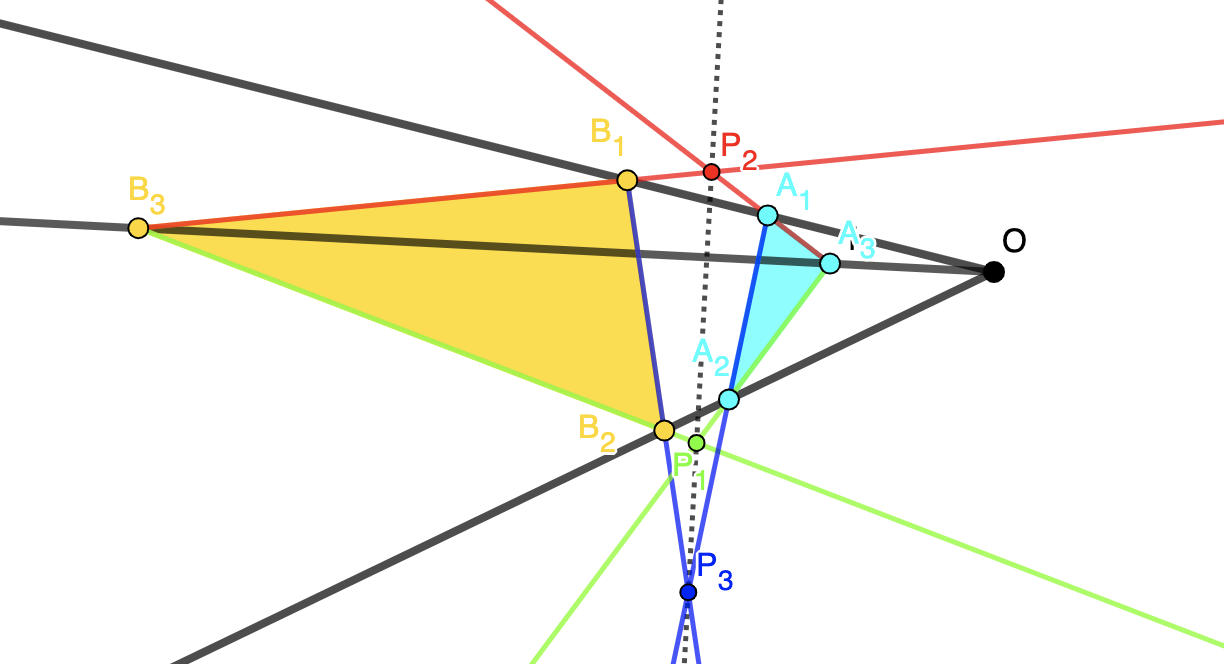
\includegraphics[scale=0.5]{Figure/05_06}
\end{figure}
\proof Essendo i vertici dei 2 triangoli a $3$ a $3$ non allineati, $P_1,P_2,P_3$ sono distinti tra di loro e distinti dai vertici.\\
I vertici $A_1, B_1, P_3,P_2$ sono in posizione generale dunque essi danno luogo ad un riferimento proiettivo di $\p(V)$ dove 
$$ A_1 =[e_0] \,\, B_1=[e_1] \, \, P_3=[e_2] \, \, P_2=[e_0+e_1+e_2]$$
Ora con un conto analogo all'esercizio~\ref{ex1} si mostra che 
$A_2=[ b, 0 , c]$ con $b,c\neq 0$ essendo $A_2\neq A_1\neq P_3$ dunque otteniamo $$A_2=[1, 0, a_2]$$ con $a_2\neq 0$\\
Ragionando in modo analogo otteniamo 
$$ A_3 = [ a_3,1,1] \text{ con } a_3\neq 0$$
$$ B_2=[0,1,b_2]\text{ con } b_2\neq 0$$
$$ B_3=[1,b_3,1]\text{ con } b_3\neq 0$$
Consideriamo i punti $$P_1'=L(A_2,A_3) \cap L(P_2,P_3)$$
$$P_1''=L(B_2,B_3)\cap L(P_2,P_3)$$
Allora $P_1,P_2,P_3$ sono allineati se e solo se 
$P_1=P_1'=P_1''$
infatti 
\begin{itemize}
\item Se $P_1,P_2,P_3$ sono allineati, $P_1\in L(P_2,P_3)$ da cui si ha $P_1=P_1'=P_1''$
\item Se $P_1=P_1'=P_1''$ allora $P_1\in L(P_2,P_3)$ 
\end{itemize}
Osserviamo che le coordinate omogenee di questi nuovi punti sono 
$$ P_1'= [1,1,1-a_2a_3+a_2]$$
$$P_1''=[1,1,1-b_2b_3+b_2]$$
Dunque si ha $P_1,P_2,P_3$ allineati se e solo se $P_1'=P_1''$ dunque se e solo se
\begin{equation}
\label{cond1}
a_2(1-a_3) = b_2(1-b_3)
\end{equation}
Esaminiamo le condizioni che fanno si che $T_1,T_2$ sono in prospettiva, ovvero sotto quali ipotesi 
$$\exists O=L(A_1,B_1) \cap L(A_2,B_2) \cap L(A_3,B_3)$$
ovvero 
$$ \begin{cases} x_2=0\\
a_2 x_2+ b_2 x_1-x_2 =0\\
(1-b_3) x_0 + (1-a_3) x_1 + (a_3b_3-1) x_2=0
\end{cases}$$
Tale soluzione ammette una soluzione non nulla se e solo se 
$$\det \begin{pmatrix}
0 & 0 & 1 \\
a_2 & b_2 & -1 \\
1-b_3 & 1-a_3 & a_3b_3-1
\end{pmatrix}=0$$
ovvero se e solo se 
$$b_2(1-b_3) = a_2(1-a_3)$$
che \`e la condizione~\ref{cond1}
\endproof
\end{thm}

\end{document}
